\documentclass{article}

% Language setting
% Replace `english' with e.g. `spanish' to change the document language
\usepackage[english]{babel}

% Set page size and margins
% Replace `letterpaper' with `a4paper' for UK/EU standard size
\usepackage[letterpaper,top=2cm,bottom=2cm,left=3cm,right=3cm,marginparwidth=1.75cm]{geometry}

% Useful packages
\usepackage{amsmath}
\usepackage{graphicx}
\usepackage[colorlinks=true, allcolors=blue]{hyperref}
\usepackage{float}
\usepackage[table,xcdraw]{xcolor}

\title{Desenvolvimento de sistema inteligente para localização e monitorização de incêndios florestais}
\author{Nuno Pires}

\begin{document}
\maketitle

\begin{center}
Repositório\\
\url{https://github.com/nunopires-uc/Fireloc}
\end{center}


\section{Data Sources}
\begin{itemize}
    \item Variety of Portugal GIS datasets from the Linking Landscape, Environment, Agriculture and Food - Green and Blue Infrastructures", Instituto Superior de Agronomia and other sources. Shapefiles or geoTiff in EPSG:3763, ETRS89/Portugal TM06, metadata in xml format, layout and a map preview. \url{http://epic-webgis-portugal.isa.ulisboa.pt/data#relevo}
    \item Geocatalogo - Catálogo com informação geográfica de dados abertos (opendata) disponível para descarregar em diversos formatos \url{https://geocatalogo.icnf.pt/catalogo_tema2.html}
    \item Informações sobre Incêndios até 2015 \url{https://github.com/centraldedados/incendios/tree/master}
    \item \url{https://prociv.gov.pt/pt/avisos-legais/acesso-a-informacao/}
    \item \url{https://effis.jrc.ec.europa.eu/applications}
\end{itemize}

\section{O que foi feito}
\subsection{Semana 23/10/23 - Resumo}
Os fatores que contribuem para o inicio de um incêndio florestal são:  \textbf{Topografia} (Elevação, Inclinação), \textbf{Tipo de Vegetação} (existem tipos de vegetação que são mais suscetíveis ao fogo), \textbf{Meteorologia}, \textbf{Fatores Humanos}, \textbf{Distância a estradas}, \textbf{Distâncias a povoações}. 


As variáveis de previsão dividem-se nas categorias: \textbf{fatores meteorológicos}, \textbf{fatores temporais}, \textbf{fatores populacionais}, \textbf{fatores paisagísticos}, \textbf{fatores de origem humana} \ref{sec:main_forest_fire_indicators}.


A previsão dos fogos florestais, além dos métodos de machine learning, podem ser previstos através de modelos matemáticos como o \textbf{FWI}.


A incidência de chuva não tem uma \textbf{correlação} muito forte com as outras variáveis meteorológicas.


A auditoria dos fogos florestais pode ser feita através do uso de ferramentas \textbf{GIS}, onde se usa vários mapas, e temas para analisar o estado do terreno, solo, vegetação e árvores. Este tipo de análise pode ser útil numa fase inicial de auditoria, e previsão das condições que culminam no inicio de um incêndio.


\subsection{Questões 23/10/23}

\subsubsection{Repartição de Informação}
O meu pensamento inicial foi atribuir a cada ocorrência de incêndio, a temperatura, e os dados geográficos correspondentes, ver exemplo \href{https://drive.google.com/file/d/13fw-uWtUAH4MEGPvmtnrrzJ5M7Pa4_cf/view?usp=sharing}{dataset 2015} e \href{https://drive.google.com/file/d/14O13kv_9zqOzVZgREm5C9k1rYZwEg72l/view?usp=sharing}{dataset 2017}.


Isto iria criar um dataset muito desbalanceado, onde teremos localidades com muito mais ocorrências que outras, o que é bom para fins estatísticos, mas não a nível de encontrar as variáveis que contêm o cerne para que aconteca a ignição de um fogo florestal.
Cada localidade pode-se encaixar num tipo de terreno, onde cada terreno partilha características comuns como é demonstrado na figura \ref{fig:tipos_de_terreno}.


Assim, era possível criar métodos, e matrizes de correlação para prever a eficácia das variáveis independentes.


Na figura \ref{fig:db_schema}, e na tabela \ref{tabela:exemplo_dataset}, está demonstrado de forma muito simplificada como seria o schema da base de dados.


A minha questão, é se esta linha pensamento é acertiva, estarmos a utilizar o tipo de terreno com as suas características (inclinação, vegetação, espécies de árvores) em vez da localidade.



\subsubsection{Outras questões}
\begin{enumerate}
    \item Deveria escrever em Português ou Inglês?
\end{enumerate}


\begin{figure}[H]
 \centering
  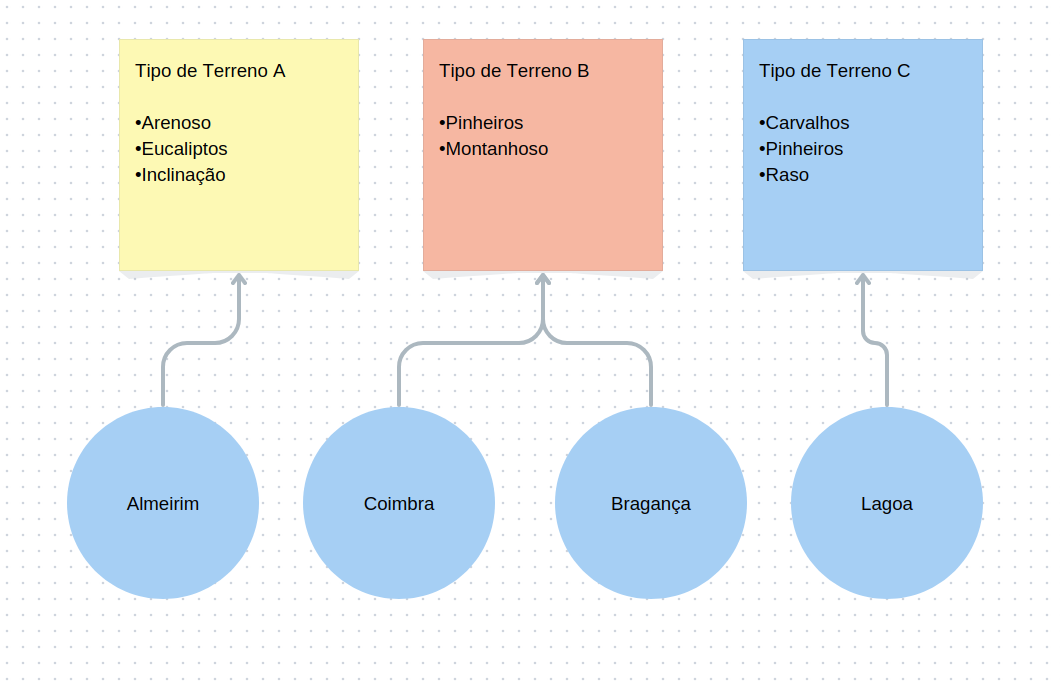
\includegraphics[width=1.0\linewidth]{imgs/tipo_de_terreno.png}
   \caption{\label{fig:tipos_de_terreno}Tipos de Terrenos}
\end{figure}

\begin{figure}[H]
 \centering
  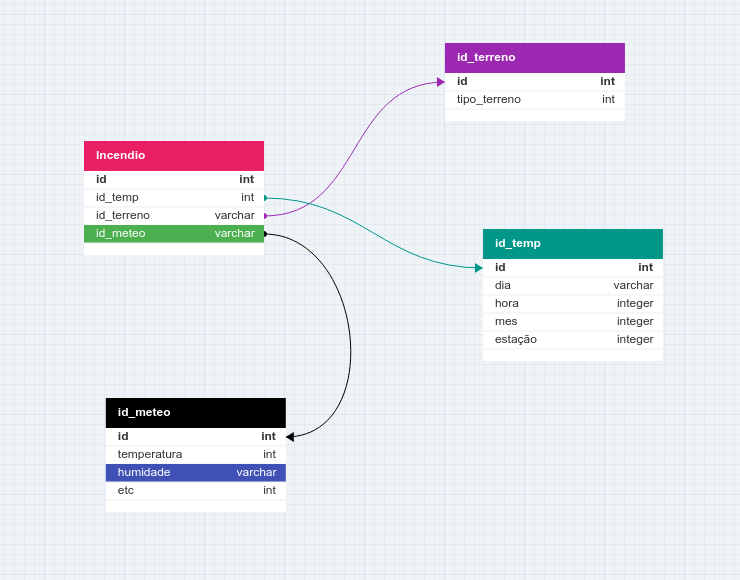
\includegraphics[width=1.0\linewidth]{imgs/db_schema.png}
   \caption{\label{fig:db_schema}Mockup schema relacional snippet base de dados}
\end{figure}

\begin{table}[H]
\label{}
\begin{tabular}{|l|l|l|l|}
\hline
\cellcolor[HTML]{FFCCC9}Codigo & \cellcolor[HTML]{ECF4FF}hora,dia,mes & \cellcolor[HTML]{FFCE93}tipo de terreno & \cellcolor[HTML]{CBCEFB}dados meteorológicos \\ \hline
1                              & 12/10/2020 15:31 outono              & A                                       & 37ºC                                         \\ \hline
2                              & 03/07/2020 13:21 verão               & C                                       & 41ºC                                         \\ \hline
3                              & 22/08/2020 10:15 verão               & A                                       & 32ºC                                         \\ \hline
\end{tabular}
\caption{\label{tabela:exemplo_dataset}Snippet exemplo tabela base de dados}
\end{table}

\section{Mapping Forest Fire Risk—A Case Study in
Galicia (Spain) \cite{Novo2020MappingFF}}
\label{sec:Mapping Forest Fire Risk—A Case Study in Galicia}

\subsection{Fatores que Contribuem para o ínicio de um incêndio e propagação}
\begin{enumerate}
\item topografia (elevação, e inclinação)
\item vegetação
\item meteorologia
\item fatores humanos
\item distância a estradas
\item distância a povoações
\end{enumerate}

\subsection{Tipos de Risco}
\begin{enumerate}
\item Risco a longo prazo: define-se pelas componentes de um território que não variam a longo prazo como a topografia, e o tipo de vegetação.
\item Risco a curto prazo: define-se por fatores que mudam, como as condições do clima.
\end{enumerate}
Risco de Incêncido define-se como a probabilidade de de ocorrência de um fogo florestal, e o dano, que potencialmente, pode vir a causar num lugar(Vulnerabilidade).
Três categorias de controlo de incêndio: Predição, monitoramento, e predição.

\subsection{Fire Weather Index} 
Componente do sistema canadiano de classificação do perigo de incêndio florestal. Neste artigo, foi usado para avaliar o perigo de incêndio, que tem em conta os efeitos da humidade do combustível.

\begin{enumerate}
    \item Temperatura (◦C)
    \item Direção do Vento(◦)
    \item Velocidade do Vento(km/h)
    \item Humidade relativa(%)
    \item Pressão absoluta(hPa)
    \item Chuva instantânea (mm)
    \item Precipitação acumulada nas últimas 24h
\end{enumerate}

\subsection{Problemas Antropogénicos}
Atividades humanas estão associadas com a ocorrência de fogo florestal, e a proximidade com as áreas urbanas, e estradas.


\section{To Predict the Fire Outbreak in Australia using 
Historical Database \cite{9964603}}
\label{sec:To Predict the Fire Outbreak in Australia using Historical Database}
Neste artigo, é usado uma abordagem de Árvores de Decisão para construir o modelo de previsão. Os datasets utilizados são da NASA'S FIRMS (Fire Information for Resource Management System) satellite data, da NASA MODIS e VIIRS dataset, e contém dados de incêndios dos últimos 20 anos.\par
O fogo florestal produz poluição de partículas finas de ar que impacta directamente a saúde humana, mesmo com pouca exposição.\par
Os prados e florestas são susceptíveis ao fogo do que
outros tipos de vegetação.\par
Zonas tropicais contém o maior número de ocorrências de incêndio, existindo um padrão de frequência sazonal.



\section{Environmental Fire Hazard Detection and 
Prediction using Random Forest Algorithm \cite{9726029}}
\label{sec:Environmental Fire Hazard Detection and Prediction using Random Forest Algorithm}
Este artigo utiliza dados dos incêndios do parque natural de Montesinho em Trás-os-Montes guardados ao longo de três anos.
A previsão meteorológica é usada para prever condições climáticas favoráveis ao acontecimento de fogos florestais.

\subsection{Parâmetros do Dataset}
\begin{enumerate}
    \item X x-axis spatial coordinate within the Montesinho park map: 1 to 9
    \item Y y-axis spatial coordinate within the Montesinho park map: 2 to 9
    \item Month Month of the year: ‘Jan’ to ‘Dec’
    \item Day Day of the week: ‘Mon’ to ‘Sun’
    \item FFMC Fine Fuel Moisture Code (FFMC)
    \item Fire Weather Index (FWI) system: 18.7 to 96.20
    \item DMC Duff Moisture Code (DMC) index from the FWI system: 1.1 to 291.3
    \item DC Drought Code (DC) index from the FWI system: 7.9 to 860.6
    \item ISI Initial Spread Index (ISI) index from the FWI system: 0.0 to 56.10
    \item Temp Temperature in Celsius degrees: 2.2 to 33.30
    \item RH Relative humidity in %: 15.0 to 100
    \item Wind Wind speed in km/h: 0.40 to 9.40
    \item Rain Outside rain in mm/m2 : 0.0 to 6.4
    \item Area Burned area of the forest (in ha): 0.00 to 1090.84
\end{enumerate}


\begin{figure}[H]
 \centering
  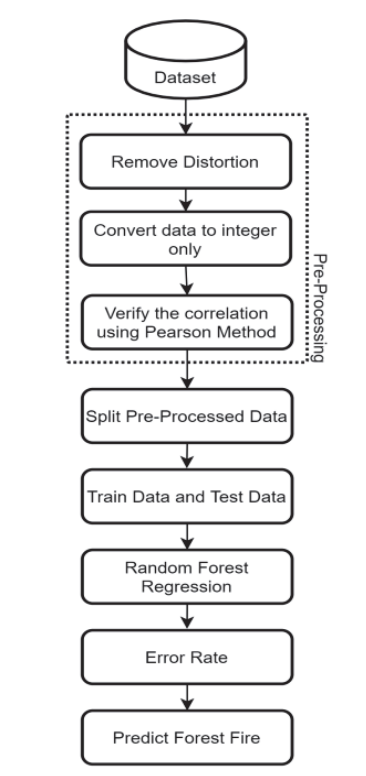
\includegraphics[width=0.25\linewidth]{imgs/flow_chart_detect_fire.png}
   \caption{\label{fig:flow_chaft}Pipeline desde o dataset à predição}
\end{figure}

\begin{figure}[H]
 \centering
  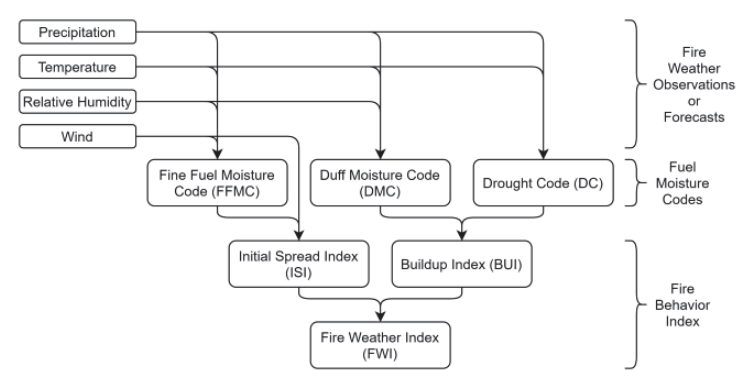
\includegraphics[width=0.70\linewidth]{imgs/fwi_structure.png}
   \caption{\label{fig:fwi_structure}Atributos meteorológicos, relações, e códigos}
\end{figure}


\subsection{Conclusões}
\begin{enumerate}
    \item A temperatura é diretamente proporcional ao mês, FFMC, DMC, DC, e ISI;
    \item Chuva e temperatura demonstram uma ausência de correlação;
    \item Chuva e FFMC demonstram uma ausência de correlação;
    \item Existe uma forte relação entre DC e o mês;
    \item A chuva não tem uma correlação muito forte com as outras variáveis.
\end{enumerate}

The Random Forest regression means the absolute error 
is 0.6664, and the Random forest regression score is 0.9799.



\section{Forest Fire Probability Prediction based on Humidity and Temperature \cite{10085661}}
\label{sec:Forest Fire Probability Prediction based on Humidity and Temperature}
Este artigo focava na humidade, oxigénio, e temperatura para a previsão. Foi criada uma aplicação onde se inseria estes três valores, e o depois, mostrado a probabilidade de ocorrer um incêndio.   
\subsection{Methodology - Passos para a previsão}
\begin{enumerate}
\item Acquisition of Dataset
\item Data preprocessing: Data Cleaning - Remove any missing or irrelevant data and ensure that the data is in a consistent format, Data Normalization - Normalize the data to ensure that all the variables have similar scales and ranges, Data Splitting - Split the data into training and testing sets to ensure that the model is trained and evaluated on different data and Data Transformation - Transform the data into a format suitable for modeling, such as converting categorical variables into numerical ones.
\item Feature Extraction: Extract relevant features such as average temperature, average humidity, and others to build a predictive model.
\item Building the model: split the data into training and testing sets. Choose an appropriate machine learning
algorithm for the prediction of forest fire probability.
\item Validation and testing
\end{enumerate}

\subsection{Vantagens de Implementação do sistema}
\begin{enumerate}
    \item Improved Accuracy: The use of machine learning algorithms allows the system to make more accurate predictions based on historical data.
    \item Early Warning: The system provides early warning of potential forest fires, allowing authorities to take preventive measures to reduce the risk of fire.
    \item Real-Time Predictions: The system provides real-time predictions based on current temperature and humidity values, which is critical in the prediction of forest fires.
    \item Cost-Effective: The proposed system is cost-effective compared to traditional methods of monitoring and predicting forest fires, which often rely on manual labor.
    \item Automated: The system is automated, reducing the need for manual intervention and increasing efficiency.
    \item Data-Driven: The system is data-driven, allowing for continuous improvement of the predictive model based on new data.
\end{enumerate}

\subsection{Conclusões}
\begin{enumerate}
    \item Muita humidade e baixas temperaturas estão a associadas a uma baixa probabilidade de ocorrência de incêndio.
    \item O uso de apenas três variáveis não é suficiente para prever fogo florestal, é necessário conjugar com a velocidade do vento, topografia, e tipo de vegetação.
\end{enumerate}


\section{Optimization of Geographic Information Systems 
for Forest Fire Risk Assessment \cite{9167162}}
\label{sec:Optimization of Geographic Information Systems for Forest Fire Risk Assessment}
The performed geographic information systems optimization enables easier and faster forecasting of critical points that could be threatened by fire
\begin{enumerate}
    \item Creating thematic layers - represent land use, population density, vegetation types, elevation, etc.
    \item Spatial analysis (understanding the relationships between geographic features or datasets) and creation of thematic maps.
    \item Development of a digital terrain model and analysis of orographic (study of the topographic relief of mountains) features relevant to the rate and direction of fire.
    \item Analysis of matrix substrate and soil type.
    \item Analysis of socio-demographic traits.
spread;
\end{enumerate}


\section{A smart approach for fire prediction under uncertain
conditions using machine learning \cite{Sharma2020}}

Estudo realizado num dataset que continha 517 instâncias e 13 atributos, mas apenas 2 atributos, temperatura e humidade relativa foram considerados.

\begin{figure}[H]
 \centering
  \includegraphics[width=0.80\linewidth]{imgs/tabela_resultados_previsão.png}
   \caption{\label{fig:model_comparison}Comparação entre os 8 modelos}
\end{figure}

O AUC demonstra o a efetividade de um modelo para distinguir entre casos correspondentes a fogo, e a casos sem fogo. Quanto maior o AUC, melhor é o modelo a fazer a distinção.


\section{Role of Machine Learning Algorithms in Forest Fire 
Management: A Literature Review \cite{arif2021role}}
\label{sec:Role of Machine Learning Algorithms in Forest Fire Management: A Literature Review}
\subsection{Áreas de Pesquisa Relacionadas com fogos Florestais}
\begin{itemize}
    \item Prediction of Fire Occurrence (time and location)
    \item Detection of already started fire event
    \item Prediction of Spread of Wildfire (burned area in future)
    \item Detection of Burned Area due to fire
\end{itemize}

\subsection{Pipeline desde a recolha de dados à aplicação do modelo}
\begin{figure}[ht]
 \centering
  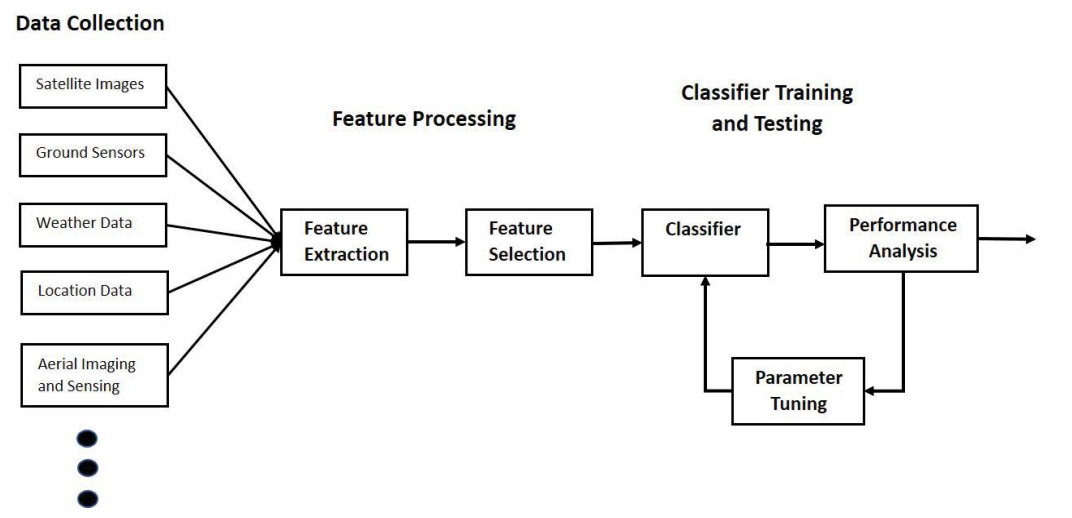
\includegraphics[width=0.80\linewidth]{imgs/pipelina_data_ml.png}
   \caption{\label{fig:pipeline_modelo}Pipeline modelo}
\end{figure}

\subsection{Fatores principais da ignição de fogos florestais}
\label{sec:main_forest_fire_indicators}
\subsubsection{Fatores Meteorológicos}
\begin{itemize}
    \item Temperatura
    \item Humidade relativa
    \item Precipitação
    \item Velocidade do Vento
    \item Trovoada
\end{itemize}

\subsubsection{Fatores Temporais}
\begin{itemize}
    \item Estação
    \item Mês
    \item Hora do dia
\end{itemize}

\subsubsection{Fatores Populacionais}
\begin{itemize}
    \item Densidade populacional
    \item Atividades humanas na floresta
    \item Comportamentos humanos
\end{itemize}

\subsubsection{Fatores Populacionais}
\begin{itemize}
    \item Densidade populacional
    \item Atividades humanas na floresta
    \item Comportamentos humanos
\end{itemize}

\subsubsection{Fatores paisagísticos}
\begin{itemize}
    \item Tipos de árvores
    \item Declive
    \item Distãncia de terrenos agrícolas
\end{itemize}

\subsubsection{Fatores de origem humana}
\begin{itemize}
    \item Curtos-circuitos nas linhas da rede elétrica que atravessam a floresta
\end{itemize}

\subsection{Prever a probabilidade de Fogo com base em modelos matemáticos}
\begin{itemize}
    \item Fire Weather Index (FWI)
    \item Angstrom index
    \item KBDI index
    \item Nesterov index
    \item Baumgartner index
\end{itemize}
A utilização de modelos de regressões logísticas pode ser usado para estimar os fogos causados por humanos.


\bibliographystyle{plain}
\bibliography{referencias}

\end{document}